\documentclass[11pt]{beamer}
\usepackage[utf8]{inputenc}
\usepackage[spanish]{babel}
\usepackage{multicol}
\usepackage{amsmath}
\usepackage{amsfonts}
\usepackage{amssymb}
\usepackage{graphicx}
\usepackage{lipsum}
\usepackage{ragged2e}
\usepackage{hyperref}
\usepackage{float}
\usepackage{url}
\usetheme{Madrid}
\newcommand{\celda}[1]{
	\begin{minipage}{2.5cm}
		\vspace{5mm}
		#1
		\vspace{5mm}
	\end{minipage}
}

\author[Abarca, Apari, Suca, Vargas] % (optional)
{J.~P.~Abarca\inst{1} \and C.~T.~Apari\inst{1} \and C.~A.~Suca\inst{1} \and A.~Vargas\inst{1}  }
\title[Practica4]{Práctica 4}
\date{ 20 de Agosto del 2021} 
%\date{\currenttime}
\subtitle{Variantes de las Máquinas de Turing e Indecibilidad}
\logo{
\includegraphics[scale=0.16]{unsa.png}}
\institute[UNSA]{
	\inst{1}
		Universidad Nacional del San Agustín. Facultad de Producción y Servicios. \\Escuela Profesional de Ciencias de la Computación\\
		Maestría en Ciencias de la Computación \\ Docente: Dra. Marcela Quispe Cruz\\
		\vspace{2mm}
}

\AtBeginSection[]
{
	\begin{frame}<beamer>{Contenido}
		\tableofcontents[currentsection,currentsubsection]
	\end{frame}
}


\begin{document}
	
	\begin{frame}
		\maketitle
	\end{frame}

	\begin{frame}{Contenido}
		\tableofcontents
	\end{frame}

	\section{Variantes de las Máquinas de Turing}
		\begin{frame}{Variantes de Máquinas de Turing}
			\justifying
			
			Presentamos los diversos tipos o variantes de Máquinas de Turing, que surgen de la necesidad de flexibilidad para la solución de problemas.\\
			Resulta que la definición de Máquina Turing(simple, normal o estándar) que analizamos es extremadamente robusta. \\
			Podemos hacer uso de las variantes de máquinas de turing, o combinarlas para obtener máquinas aún más complejas, pero ello no implica que ofrecen mayor capacidad para describir lenguajes que la versión estándar. \\
			Porque todos ellos tienen el mismo poder computacional.
			
		\end{frame}
		\begin{frame}{Máquina de Turing Estándar}
			\justifying
			
			\begin{itemize}
			    \item Determinista.
		        \item Una sóla cinta.
		        \item Un solo cabezal de lectura y escritura.
		        \item Infinito a la derecha, limitado por la izquierda.
		        \item función de transición: $\delta : Q \times \Gamma \rightarrow Q \times \Gamma \times \{ L, R \}$  \\
			\end{itemize}
		     
			\begin{figure}[H]
				\centering
				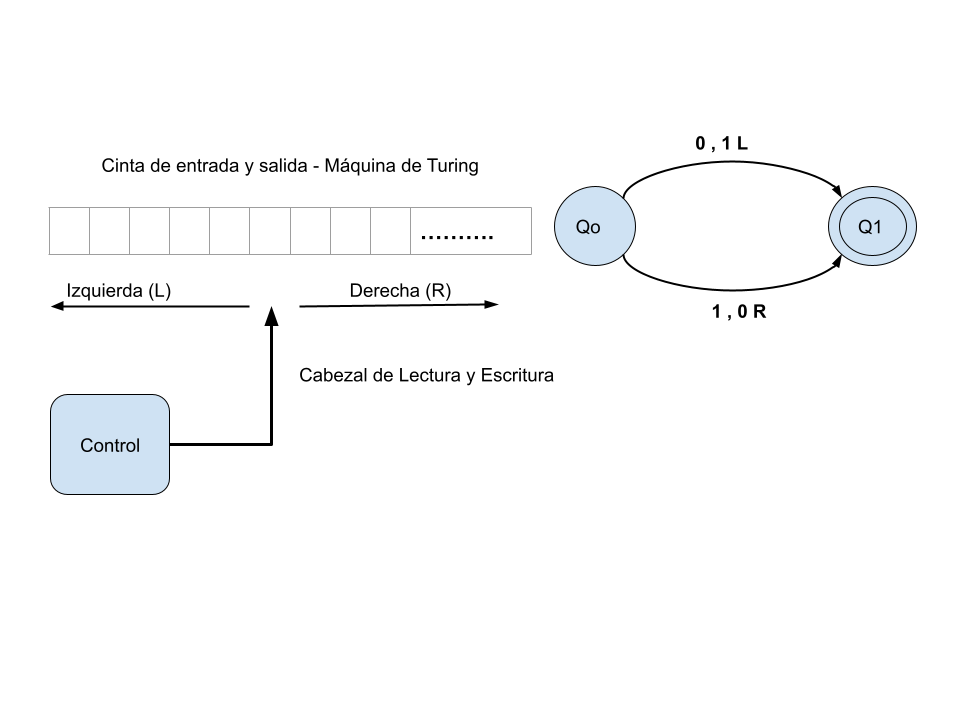
\includegraphics[scale=0.28]{img/standar.png}
				\caption{Máquina Turing Estándar y diagrama de estados}
				\label{fig: Standar}
			\end{figure}
		\end{frame}
	
	\subsection{Máquinas de Turing Stay-Put}
	    \begin{frame}{Stay-Put}
			\justifying
			
			Esta variante de máquina de Turing, tiene la capacidad de mantener el cabezal en el mismo lugar de la cinta. \\
			
			¿Podría esta característica permitir que las máquinas de Turing reconozcan lenguajes adicionales, aumentando así la potencia del modelo? Por supuesto que no, porque podemos convertir cualquier Máquina de Turing con la función de permanecer en su sitio, en una que no la tenga. \\
			Lo hacemos reemplazando cada transición fija con dos transiciones: una que se mueve hacia la derecha y la segunda hacia la izquierda o una que se mueve a la izquierda y la segunda hacia la derecha. \\
			Este pequeño ejemplo contiene la clave para mostrar la equivalencia de variantes de Máquinas de Turing con la Máquina Turing Estándar.
			
		\end{frame}
		\begin{frame}{Stay-Put - Diagrama de Estados y Función de Transición }
			\justifying
			$\delta : Q \times \Gamma \rightarrow Q \times \Gamma \times \{ L, R, S \} $\\
			
			\begin{figure}[H]
				\centering
				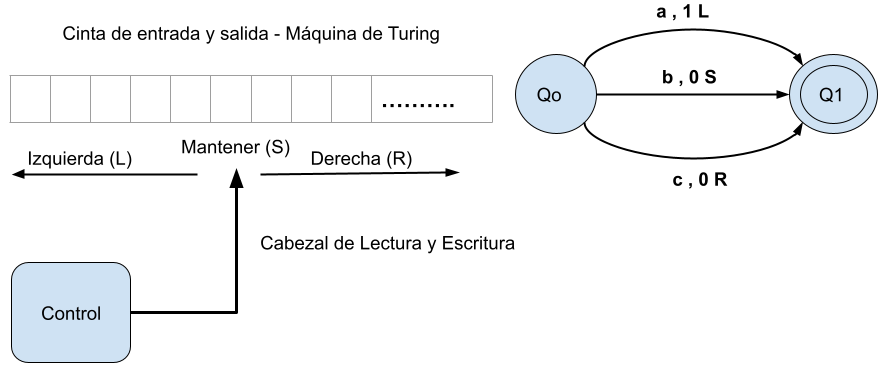
\includegraphics[scale=0.5]{img/stayput.png}
				\caption{Máquina Turing Stay-Put y diagrama de estados}
				\label{fig: Stay-Put}
			\end{figure}
			
			
		\end{frame}
	\subsection{Máquinas de Turing con cintas infinitas por ambos lados}
	
	\begin{frame}{Cintas infinitas por ambos lados}
			\justifying
			
				Una cinta infinita bidireccional de una Máquina de Turing, puede moverse indefinidamente en cualquier dirección. \\
				
				Se puede demostrar que esto es equivalente a una Máquina de Turing de cinta infinita unidireccional mediante el siguiente argumento: Está claro que se pueden usar dos Máquinas de Turing de cinta infinita unidireccional para simular una cinta infinita bidireccional. Si estos están alineados `` uno al lado del otro '' y las dos cintas están intercaladas, entonces se puede construir una sola Máquina de Turing infinita unidireccional que sea equivalente.
	
	
		\end{frame}
		
	    \begin{frame}{Cintas por ambos lados - Diagrama de Estados y Función de Transición}
			\justifying
			
			\begin{figure}[H]
				\centering
				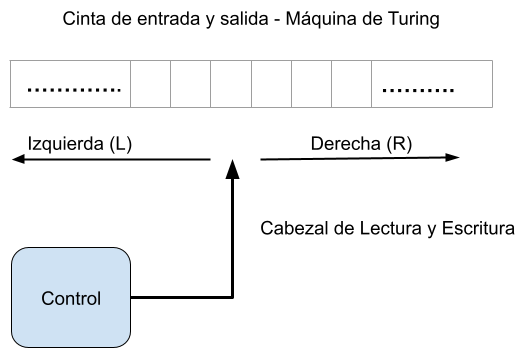
\includegraphics[scale=0.35]{img/infiniteside.png}
				\caption{Máquina Turing cintas infinitas y diagrama de estados}
				\label{fig: InfiniteSide}
			\end{figure}
			
		\end{frame}
	

	
	\subsection{Máquinas de Turing Multicabezal}
	    \begin{frame}{Multicabezal}
			\justifying
			
			Esta es una Máquina de Turing de una sola cinta con múltiples cabezales de lectura / escritura. \\
			En cada estado solo se puede usar una cabeza. \\
			Por lo tanto, para k cabezas
tienen una partición de los estados Q1, Q2,. . . , Qk donde cada Qi contiene el conjunto de estados que utilizan el i-ésimo
cabeza. 
			
		\end{frame}
	\begin{frame}{Multicabezal - Diagrama de Estados y Función de Transición }
			\justifying
			$\delta : Q  \times \{ H1 , H2 ... , Hn \}  \times (\Gamma \cup \{ \Delta\}) \rightarrow  (Q \cup \{ h \}) \times (\Gamma \cup \{\Delta\}) \times \{R,L,S\}$ \\ 
			Donde H1,H2, ..., Hn, representan los cabezales. \\
			\begin{figure}[H]
				\centering
				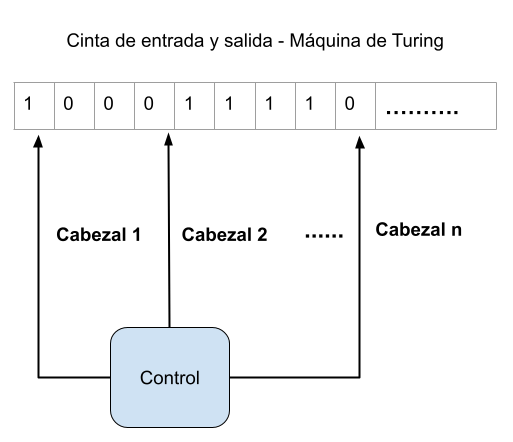
\includegraphics[scale=0.35]{img/mulltihead.png}
				\caption{Máquina Turing MultiCabezal y diagrama de estados}
				\label{fig: MultiHead}
			\end{figure}
			
			
		\end{frame}
	\subsection{Máquinas de Turing Multidimensional}
	    \begin{frame}{Multidimensional}
			\justifying
			
			Este es un tipo de máquinas de Turing que tienen un control finito, un cabezal de lectura y escritura y una cinta bidimensional, extendiéndose hacia la derecha y hacia abajo infinitamente. \\
			Para cualquier máquina de Turing de este tipo existe una máquina de Turing con una cinta unidimensional igualmente potente, es decir, la primera puede ser simulada por la segunda. 
			
		\end{frame}
		\begin{frame}{Multidimensional - Diagrama de Estados y Función de Transición }
			\justifying
			$\delta : Q \times \Gamma \rightarrow Q \times \Gamma \times \{ L, R, U,D \}$ \\
			\begin{figure}[H]
				\centering
				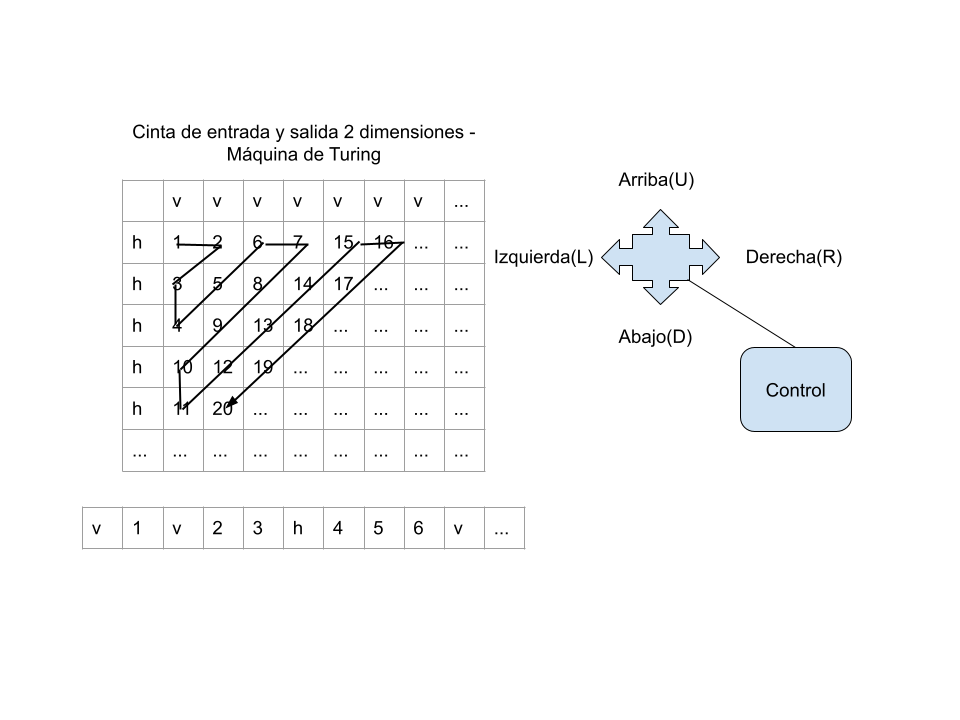
\includegraphics[scale=0.30]{img/multidimensional.png}
				\caption{Máquina Turing 2-Dimensional y diagrama de estados}
				\label{fig: MultiDimensional}
			\end{figure}
			
			
		\end{frame}
	
	\subsection{Máquinas de Turing con Múltiples Tracks}
	    \begin{frame}{Múltiples Tracks}
			\justifying
			Contienen varias pistas, pero solo un cabezal de cinta que lee y escribe en todas las pistas.\\
			Aquí, un solo cabezal de cinta lee n símbolos de n pistas en un solo paso. \\
			
			Para cada Máquina Turing S de una sola pista, hay una máquina Máquina de Turing con múltiples tracks equivalente tal que L(S) = L(M).
			
		\end{frame}
	    \begin{frame}{Múltiples Tracks - Diagrama de Estados y Función de Transición}
			\justifying
			
			$\delta(q_{i},[x1,x2, . . . , xn]) = (q_{j} , [y1, y2, . . . , yn],L)$ \\
			
			\begin{figure}[H]
				\centering
				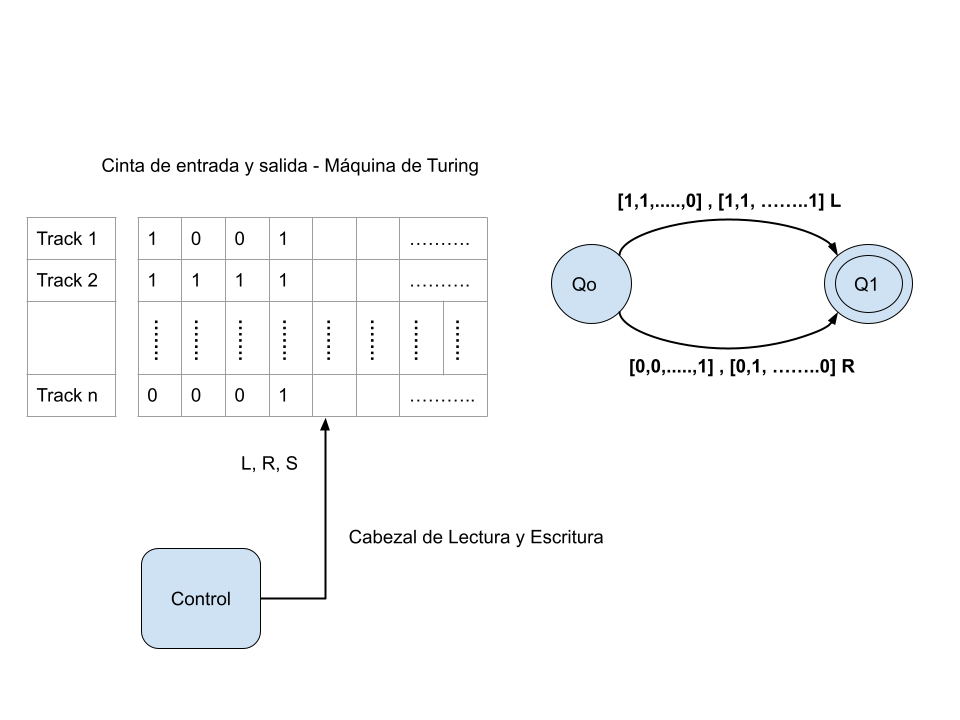
\includegraphics[scale=0.28]{img/multitracks.png}
				\caption{Máquina Turing Múltiples Tracks y diagrama de estados}
				\label{fig: Multitracks}
			\end{figure}
		\end{frame}
	\subsection{Máquinas de Turing Multicinta}
	    \begin{frame}{Multicinta}
			\justifying
			
			Esta variante consta de múltiples cintas, cada una tiene su propio cabezal. Inicialmente la 	primera cinta contiene la entrada, las demás inician en blanco. \\
			La función de transición se cambia para permitir leer, escribir y mover los cabezales en algunas o todas las cintas 	simultáneamente. \\
			Las máquinas de Turing de cintas múltiples parecen ser más poderosas que las máquinas de Turing estándar, pero podemos demostrar que son equivalentes en potencia. Recuerde que dos máquinas son equivalentes si reconocen el mismo lenguaje.\\

            Teorema 3.13. Cada máquina de Turing de varias cintas tiene una máquina de Turing de una sola cinta equivalente.
			
		\end{frame}
		\begin{frame}{Multicinta - Diagrama de Estados y Función de Transición }
			\justifying
			$\delta : Q \times \Gamma^k \rightarrow Q \times \Gamma^k \times \{ L, R, S \}^k$ \\
			
			Donde K es el número de cintas.\\
			$\delta(q_{i}, a1, . . . , ak) = (q_{j} , b1, . . . , bk,L, R, . . . ,L)$ \\
			
			
			\begin{figure}[H]
				\centering
				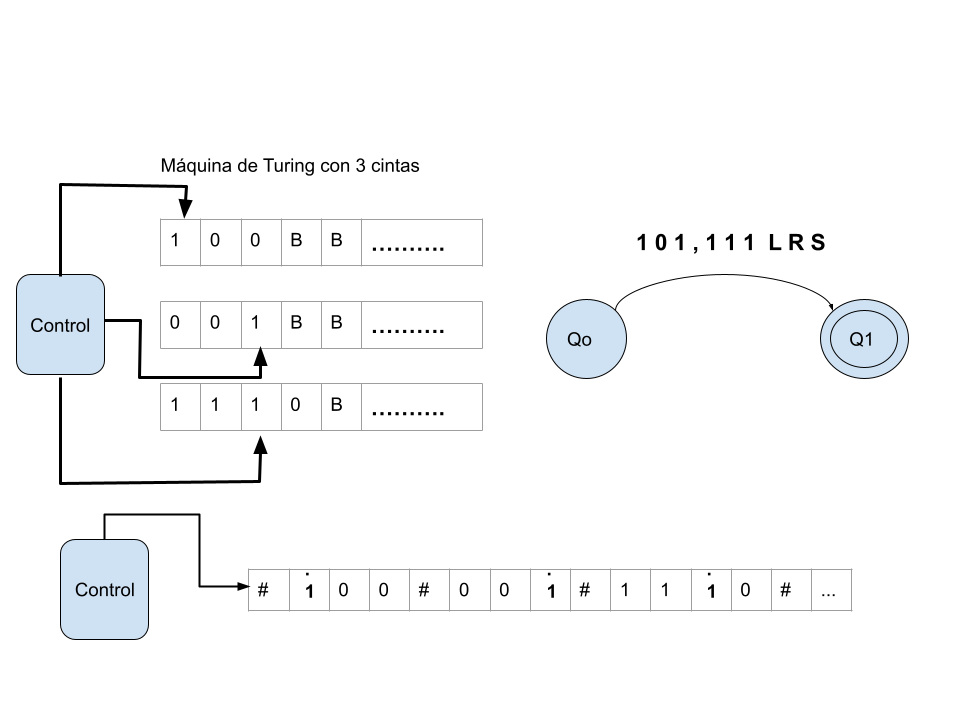
\includegraphics[scale=0.27]{img/multitape.png}
				\caption{Máquina Turing y diagrama de estados}
				\label{fig: MultiTape}
			\end{figure}
		\end{frame}
		
	\subsection{Máquinas de Turing no Deterministas}
	    \begin{frame}{Máquinas de Turing no Deterministas}
			\justifying
			
			La máquina de Turing puede proceder con muchas posibilidades, la función de transición para una maquina de turing no deterministica \cite{jflap} se da la siguiente forma:
			
			$\delta: Q x \Gamma \rightarrow P(Q x \Gamma  x \{L,R\})$
			
			 
			\begin{center}
            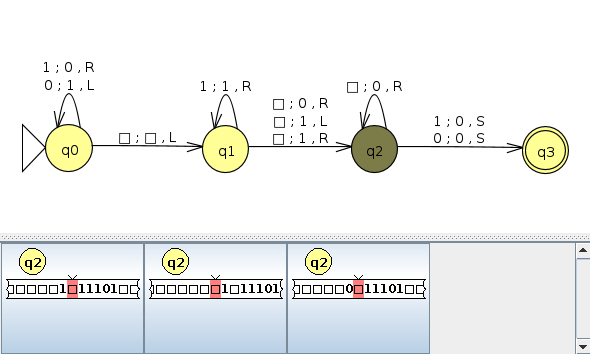
\includegraphics[scale=0.4]{img/nodet_mt.png}
			\end{center}
			
		\end{frame}
		
		\begin{frame}{Máquinas de Turing no Deterministas}
			\justifying
			
			\begin{theorem}
                Cada MT No determinista tiene un equivalente de MT determinista.
            \end{theorem}
            \begin{center}
            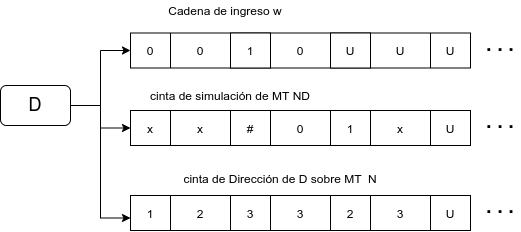
\includegraphics[scale=0.6]{img/teo1_nd.png}
			\end{center}
			
		\end{frame}

        \begin{frame}{Máquinas de Turing no Deterministas}
			\justifying
            \begin{theorem}
                Cada MT No determinista tiene un equivalente de MT determinista.
            \end{theorem}
            \begin{center}
            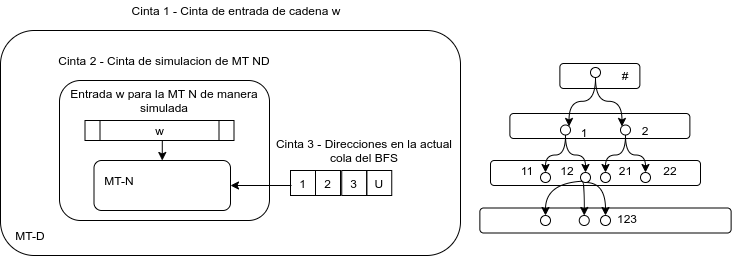
\includegraphics[scale=0.5]{img/teo1_mtn.png}
			\end{center}
		\end{frame}
		
		\begin{frame}{Máquinas de Turing no Deterministas}
			\justifying
            \begin{theorem}
                Un lenguaje es turing reconocible si y solamente si  alguna MT N reconoce esto.
            \end{theorem}
            \begin{proof}
                Cualquier MT D es automaticamente una MT N. direccion izq.
            \end{proof}
            \begin{proof}
                Cualquier MT N tiene su equivalente de MT D. direccion der
            \end{proof}
		\end{frame}
		
		\begin{frame}{Máquinas de Turing no Deterministas}
			\justifying
            \begin{definition}
                Sea $L\subseteq \Sigma^{*}$ Decimos que una MT decide L si para toda w $\in \Sigma^{*}$, la MT decide w
            \end{definition}
            \begin{definition}
                Llamamos MT N decidor si todas las ramas tiene estado de parada sobre todos los ingresos de cadenas.
            \end{definition}
		\end{frame}
		
		\begin{frame}{Máquinas de Turing no Deterministas}
			\justifying
			\begin{theorem}
                Si una MT N siempre para sobre todas sus ramas de su computación, una MT D siempre también tendrá estado de parada sea de aceptación o rechazo.
            \end{theorem}
            \begin{corollary}
                Un lenguaje es decidible si y solamente si alguna MT N decide esto.
            \end{corollary}
		\end{frame}
		
		
	\subsection{Enumeradores}
	    \begin{frame}{Lenguajes Recursivos y Recursivamente Enumerables}
			\justifying
			Recordando...
            \begin{definition}
                Lenguaje de Turing Decidible (Lenguaje Recursivo)
                \begin{itemize}
                    \item L es aceptada por una MT M
                    \item M siempre para (se detiene)
                    \item M decide L
                \end{itemize}
            \end{definition}
    	    \begin{center}
	        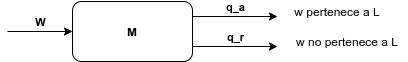
\includegraphics[scale=0.5]{img/mtdecidible_lengrec.png}
    		\end{center}
		\end{frame}
		
		\begin{frame}{Lenguajes Recursivos y Recursivamente Enumerables}
			\justifying
			Recordando...
            \begin{definition}
                Lenguaje de Turing Reconocible (Lenguaje Recursivamente Enumerable)
                \begin{itemize}
                    \item L es aceptada por una MT M
                    \item M no siempre para (Loop)
                    \item M no decide L
                \end{itemize}
            \end{definition}
    	    \begin{center}
	        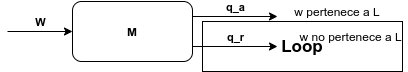
\includegraphics[scale=0.5]{img/lenTurRec_rec_enume.png}
    		\end{center}
		\end{frame}
		
	    \begin{frame}{Enumeradores}
			\justifying
            \begin{definition}
                Una lenguaje que es turing reconocible es también lenguaje recursivamente enumerable de ahí la existencia de una MT enumerable.
            \end{definition}
            Una máquina enumerable E es aquella que imprime como output todas las cadenas aceptadas por una maquina de turing

    	    \begin{center}
	        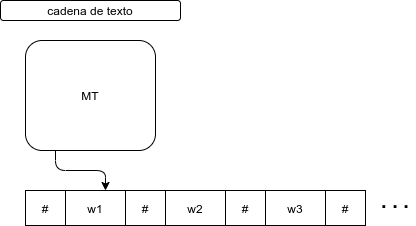
\includegraphics[scale=0.5]{img/turingmachines.png}
    		\end{center}
  
		\end{frame}
		
		\begin{frame}{Enumeradores}
			\justifying
            
            \begin{itemize}
                \item El enumerador E si no para puede imprimir infinitamente (recursivamente enumerable).
                \item Su lenguaje es una colección de cadenas que en algún momento se imprimen.
                \item las cadenas son generadas e impresas en cualquier orden
                \item las cadenas pueden imprimirse con repetición.
            \end{itemize}
		\end{frame}
		
		\begin{frame}{Enumeradores}
			\justifying
            \justifying
	        \begin{theorem}
                Un lenguaje es turing reconocible si el enumerador E (MT) enumera este.
            \end{theorem}
            \begin{proof}
                    Un enumerador E que enumera un lenguaje A, si y solo si una MT M reconoce A.
                    \begin{itemize}
                        \item M toma entrada w
                        \item Corre Enumerador, y cada vez que imprime algo se compara con w.
                        \item si w aparace en la salida de E, entonces acepta.
                    \end{itemize}
            \end{proof}
		\end{frame}
		\begin{frame}{Enumeradores - Demostracion Izq}
			\justifying
	        \begin{theorem}
                Sea $L$ es recursivamente enumerable, si y solo si  $L = G(M)$ para una máquina enumerable. 
            \end{theorem}
            \begin{center}
            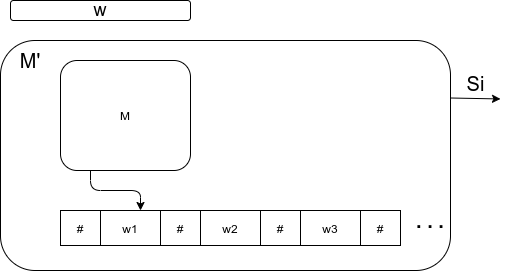
\includegraphics[scale=0.5]{img/teo1.png}
			\end{center}
		\end{frame}
		\begin{frame}{Enumeradores}
			\justifying
            \justifying
	        \begin{theorem}
                Un lenguaje es turing reconocible si el enumerador E (MT) enumera este.
            \end{theorem}
            \begin{proof}
                    Si existe un MT M que reconoce A, se puede construir un enumerador E para A, Decir que s1,s2,..,si lista de posibles strings de $\Sigma^{*}$
                    \begin{itemize}
                        \item E ignora el ingreso
                        \item Repetir para $i=1,2,...,m$
                        \item Corre MT M para i pasos sobre cada ingreso s1,s2,...,si
                        \item Si acepta alguna computacion, se imprime la correspondiente si.
                    \end{itemize}
            \end{proof}
		\end{frame}
		
		
		
		\begin{frame}{Enumeradores  - Demostracion Der}
			\justifying
	        \begin{theorem}
                Sea $L$ es recursivamente enumerable, si y solo si  $L = G(M)$ para una máquina enumerable. 
            \end{theorem}
            \begin{center}
            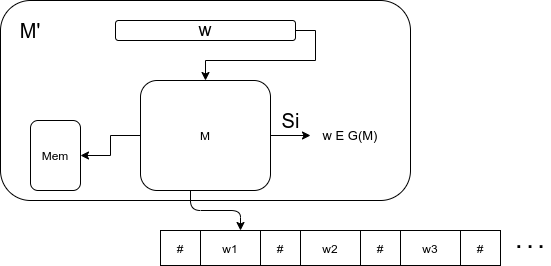
\includegraphics[scale=0.5]{img/teo1_b.png}
			\end{center}
		\end{frame}
		
		\begin{frame}{Enumeradores - Demostracion Izq}
			\justifying
	        \begin{theorem}
                Si $L$ es recursivo, si y solo si  $L$ puede ser generado en orden por una maquina de turing
            \end{theorem}
            \begin{center}
            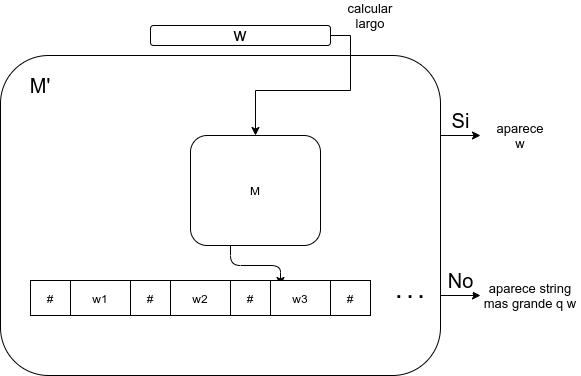
\includegraphics[scale=0.4]{img/teo_2.png}
			\end{center}
		\end{frame}
		
		\begin{frame}{Enumeradores - Demostracion Der}
			\justifying
	        \begin{theorem}
                Si $L$ es recursivo, si y solo si  $L$ puede ser generado en orden por una maquina de turing
            \end{theorem}
            \begin{center}
            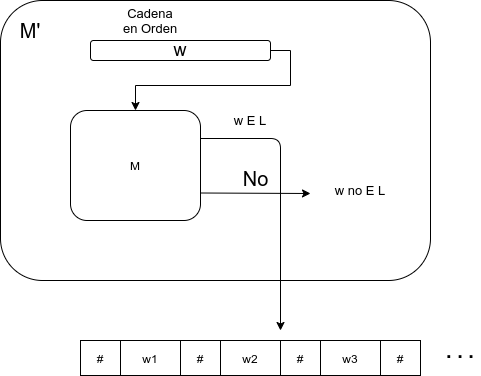
\includegraphics[scale=0.4]{img/teo2_b.png}
			\end{center}
		\end{frame}
	
	\section{Indecibilidad}
		\begin{frame}{Introducción}
			\justifying
			Turing escribió muchos programas, incluso trabajó en descifrar códigos para los ejércitos aliados durante la segunda guerra mundial. Rápidamente se dió cuenta de que algunos programas se 'colgaban' y se quedaban dando vueltas para siempre sin avanzar.\\ .
			\\
			Si queremos escribir un programa "perfecto", que nunca se cuelgue, entonces una forma de hacerlo es probarlo con todas las entradas posibles, pero esto muchas veces no es práctico porque hay demasiadas combinaciones, pero además de no ser práctico, tiene un problema más de fondo y es que aún cuando transcurra mucho tiempo nunca podemos saber si el programa está calculando todavía o si se ha quedado 'colgado'\\ .
			\\
			El principio de indecibilidad de Turing dice que no es posible escribir un programa que decida si otro programa cualquiera está correctamente escrito
		\end{frame}
		

		
		
		\begin{frame}{Teorema de la Indecibilidad}
			\justifying
			El teorema se basa en determinar si una máquina de Turing acepta una determinada cadena de entrada.\\
			Lo llamamos $A_{TM}$ por analogía con $A_{DFA}$ y $A_{CFG}$. Pero, mientras
            $A_{DFA}$ y $A_{CFG}$ fueron decidibles, $A_{TM}$ no lo es. Entonces:
            
			\begin{equation}
			    A_{TM} = \{ \langle M,w \rangle | M \text{ es una } TM \text{ y } M \text{ acepta } w \}
			\end{equation}
			
			$U=$ Entrada $\langle M,w \rangle$, donde $M$ es una MT y w es una cadena:
		    
		    \begin{enumerate}
		        \item Simulando $M$ en una entrada w
		        \item Si $M$, entra en un estado de aceptación, 'acepta'; \\
		        Si $M$, entra en un estado de rechazo, 'rechazada';
		    \end{enumerate}
			
		\end{frame}
		
		
		\begin{frame}{Flujo de un algoritmo Indecidible}
		
		    \justifying
		    
		    \begin{figure}[H]
				\centering
				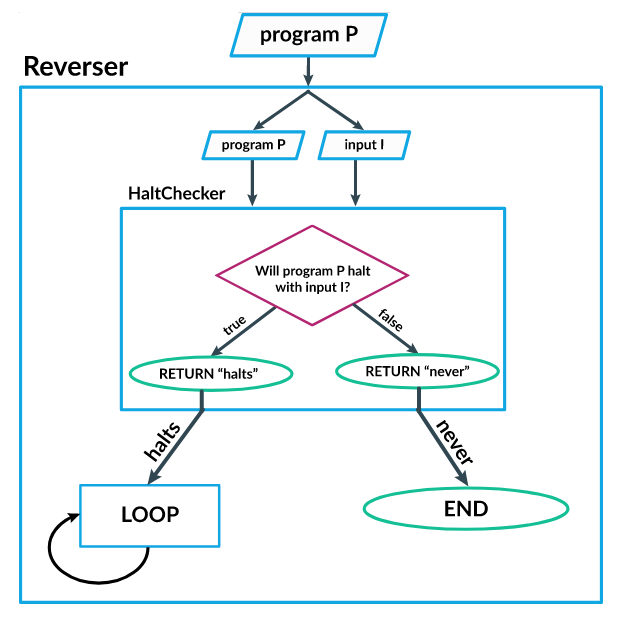
\includegraphics[scale=0.5]{img/inde_algoritmo.png}
				\caption{Flujo de Indecibilidad $L$}
				\label{fig: Flujo de Indecibilidad}
			\end{figure}
		    
		\end{frame}
		
		
		
	\subsection{Metodo de la Diagonalización}
	    \begin{frame}{Metodo de la Diagonalización}
			\justifying
			En 1873 Georg Cantor estaba preocupado
            con el problema de medir los tamaños de conjuntos infinitos. Si tenemos dos conjuntos infinitos, ¿cómo podemos saber si uno es más grande que el otro o si son del mismo tamaño? \\
            Para conjuntos finitos, es sencillo, ya que simplemente debemos contar los elementos en un conjunto finito, y el número resultante es su tamaño. Pero
            si tratamos de contar los elementos de un conjunto infinito ¡nunca terminaremos! \\
            Entonces, Cantor propuso una solución a este problema. Observó que dos los conjuntos finitos tienen el mismo tamaño si los elementos de un conjunto se pueden emparejar con el
            elementos del otro conjunto. Este método compara los tamaños de dos conjuntos infinitos sin tener que contarlos.
		\end{frame}
		
		
		\begin{frame}{Definicion de Diagonalización}
			\justifying
			Suponga que tenemos los conjuntos A y B y una función f de A a B.
            Supongamos que f es uno a uno si nunca asigna dos elementos diferentes al mismo lugar, es decir, si $f(a) \neq f(b)$ siempre que $a \neq b$. Se dice que f está en todos los elementos de B, es decir, si para cada $b \in B$ hay un $a \in A$ tal que $f(a) = b$. Tal que A y B son de igual tamaño si está de uno a uno, en la función $f: A \to B$. Una función esta representada uno sobre uno se llama correspondencia. En una correspondencia cada elemento de A se asigna a un elemento único de B y cada elemento de B tiene un elemento único de A mapeado.
            Una correspondencia es simplemente una forma de emparejar los elementos de A con los elementos de B.
		\end{frame}
		
		
		\begin{frame}{Emparejamiento I}
			\begin{multicols}{2}
			    \justifying
                Sea N el conjunto de números naturales \{1, 2, 3, ...\} y sea E el conjunto de números naturales pares \{2, 4, 6, ...\}. Usando la definición de Cantor de tamaño, podemos ver que N y E tienen el mismo tamaño. La correspondencia f mapeando N a E es simplemente f(n) = 2n
                \columnbreak
                
                \begin{figure}[H]
    				\centering
    				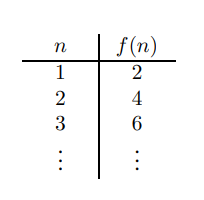
\includegraphics[scale=0.7]{img/inde_emparejam_1.png}
    				\caption{Emparejamiento de Números Pares}
    				\label{fig: inde_emparejam_1}
    			\end{figure}
                
            \end{multicols}
		\end{frame}
		
		
		\begin{frame}{Emparejamiento II}
			\begin{multicols}{2}
		        \justifying
                Si decimos que Q = \{$  \frac{m}{n}|m, n \in N$\} sea el
                conjunto de números racionales positivos, Q parece ser mucho mayor que N. Sin embargo, estos dos conjuntos son del mismo tamaño según nuestra definición. Damos una correspondencia con N para mostrar que Q es contable. Una forma sencilla de hacerlo es enumerar todos los elementos de Q. Luego emparejamos el primer elemento de la lista con el número 1 de N, el segundo elemento de la lista con el número 2 de N, y así sucesivamente.
                
                \columnbreak
                
                \begin{figure}[H]
    				\centering
    				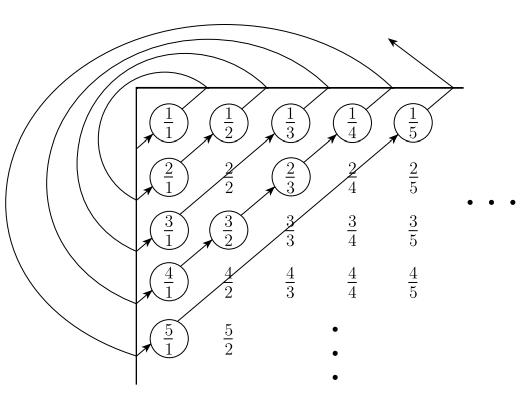
\includegraphics[scale=0.4]{img/inde_emparejam_2.png}
    				\caption{Emparejamiento de Divisibilidad}
    				\label{fig: inde_emparejam_2}
    			\end{figure}
                
            \end{multicols}
		\end{frame}
		
		
		\begin{frame}{Lenguaje de Diagonalizacion I}
			\justifying
			Supongamos una tabla infinita en la que:
			\begin{itemize}
                \item En la primera fila se colocan las cadenas de (0+1)* en orden canónico
                \item En la primera columna se colocan las Maquinas de Turing ordenadas por el orden canónico de sus codificaciones
                \item $Para: i, j \geq 1 $
                    \begin{itemize}
                        \item $ (i, j) = 1$ si la cadena j es aceptada por la maquina que se codifica en binario como $i \to w_j$ esta en $L(M_i) $
                        \item $ (i, j) = 0$ si la cadena j no es aceptada por la maquina que se codifica en binario como $i \to w_j$ esta en $L(M_i) $
                    \end{itemize}
            \end{itemize}
		\end{frame}
		
		\begin{frame}{Lenguaje de Diagonalizacion II}
		
		    \justifying
		    
		    \begin{figure}[H]
				\centering
				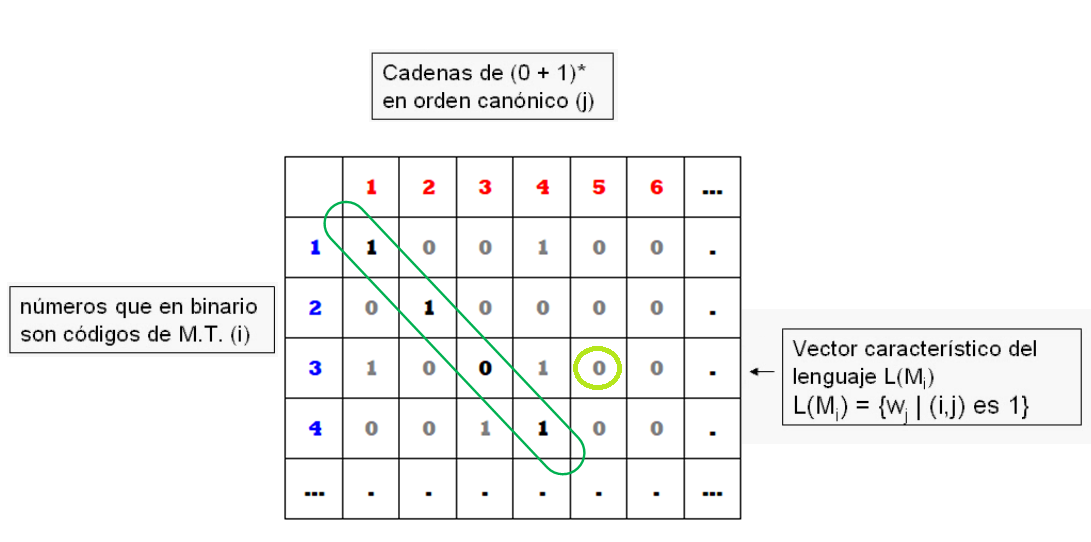
\includegraphics[scale=0.4]{img/inde_diagonaliz.png}
				\caption{Matriz de Diagonalizacion}
				\label{fig: diagonalizacion}
			\end{figure}
		    
		\end{frame}
		
		
		\begin{frame}{Lenguaje de Diagonalizacion III}
			\justifying
			Consideremos la diagonal de la tabla anterior y consideremos
			
			\begin{multicols}{2}
		        \justifying
                \begin{center}
    			    $L_d = \{ {w_i: w_i \notin L(M_i)}\}$
    			\end{center}
                
                \columnbreak
                
                \begin{itemize}
                    \item $ Si (i,i)=0, w_i \in L_d$
                    \item $ Si  (i,i)=1, w_i \notin L_d$
                \end{itemize}
                
            \end{multicols}
            
			
			\textbf{ $L_d$ no es recursivamente enumerable }
			\begin{itemize}
                \item Supongamos que si lo es $\rightarrow \exists M : L(M) = L_d$
                \item En las filas está todas las M.T. $\rightarrow \exists j : M_j = M$
                \item Entonces:
                    \begin{itemize}
                        \item Si $x_j \in L_d = L(M_j) \rightarrow (i,j)=0 \rightarrow x_j \notin L(M_j) \text{ ó } x_j \notin L_d$
                        \item Si $x_j \notin L_d = L(M_j) \rightarrow (i,j)=1 \rightarrow x_j \in L(M_j) \text{ ó } x_j \in L_d$
                    \end{itemize}
            \end{itemize}
            
            Luego no existe una MT capaz de reconocer $L_d$ y por tanto $L_d$ no es recursivamente enumerable. Luego la consecuencia de $L_d$ es:

            \begin{itemize}
                \item No recursivamente enumerable
                \item Recursivamente enumerable no recursivo
            \end{itemize}
          
            
		\end{frame}
		
	\subsection{Un Lenguaje Indecidible}
	    \begin{frame}{Un Lenguaje Indecidible}
			\justifying
			
			Considerando el Teorema inicial \cite{Sipser2013} que dice :\\
			
			\begin{theorem}
                $A_{TM}$ es indecidible
            \end{theorem}
			 ( ver ecuación \ref{eq:lenguajeIndecidible}) \\
			
			Asumimos
			
			\begin{equation} \label{eq:lenguajeIndecidible}
			    A_{TM} = \{ \langle M,w \rangle | M \text{ es una } TM \text{ y } M \text{ acepta } w \}
			\end{equation}
			
			
			\begin{proof}
                Asumimos que $H$ es un decisor para $A_{TM}$. Con la entrada $\langle M,w \rangle$ donde $M$ es una Máquina de Turing y $w$ es un string. ( ver ecuación \ref{eq:halt} )
            \end{proof}
			
			\begin{equation} \label{eq:halt}
			    H(A_{TM}) = \begin{cases}
                            aceptado & \text{ si $M$ acepta $w$ } \\
                            rechazado & \text{ si $M$ no acepta $w$. }
                        \end{cases}
			\end{equation}
			
		\end{frame}
		
		\begin{frame}{Probando que un Problema de Parada (H) es Indecidible}
		
		    \justifying
		    
		    Construir una Máquina de Turing (MT) $D$ que usa a $H$ como subrutina: Llama a $H$ para determinar como $M$ se comporta en la entrada $\langle M \rangle$ y sale el opuesto.
		    
		    $D=$ ``En el string de entrada $\langle M \rangle$, donde $M$ es una MT:
		    \setbeamertemplate{enumerate items}[default]
		    \begin{enumerate}
		        \item Ejecutar $H$ sobre la entrada $\langle M, \langle M \rangle \rangle$
		        \item Salida como el opuesto de $H$, por ejemplo si $H$ acepta, rechaza; si $H$ rechaza, acepta''.
		    \end{enumerate}
		    
		    No confundir con la noción de ejecutar una Máquina con su propia descripción, en resumen,
		    \begin{equation} \label{eq:mismo}
			    D(\langle M \rangle) = \begin{cases}
                            aceptado & \text{ si $M$ no acepta $\langle M \rangle$ } \\
                            rechazado & \text{ si $M$ acepta $\langle M \rangle$. }
                        \end{cases}
			\end{equation}
		\end{frame}
		
		\begin{frame}{Probando que un Problema de Parada (H) es Indecidible}
		
		    \justifying
		    
		    \begin{figure}[H]
				\centering
				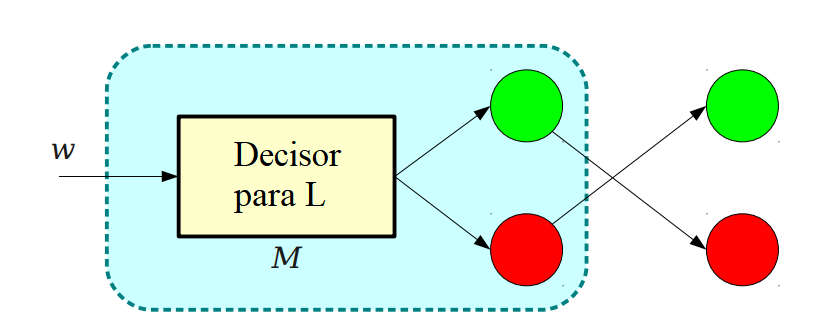
\includegraphics[scale=0.5]{img/decisorParaM.PNG}
				\caption{Ejemplo de salida opuesta a la entrada para un lenguaje $L$}
				\label{fig: DecisorParamM}
			\end{figure}
		    
		\end{frame}
		
		\begin{frame}{Probando que un Problema de Parada (H) es Indecidible}
		
		    \justifying
		    
		    ¿Que ocurriría si ejecutamos $D$ en $\langle D \rangle$ como entrada?
		    \begin{equation} \label{eq:ocurre}
			    D(\langle D \rangle) = \begin{cases}
                            aceptado & \text{ si $D$ no acepta $\langle D \rangle$ } \\
                            rechazado & \text{ si $D$ acepta $\langle D \rangle$. }
                        \end{cases}
			\end{equation}
			
			Lo que pasaria es que $D$, esta forzado a hacer lo opuesto, por lo tanto ni la MT de $D$ ni la $H$ pueden existir.
			
		\end{frame}
		
		\begin{frame}{¿Dónde esta la Diagonalización?}
		
		    \justifying
		    
		    El uso de la diagonalización puede ser visto si no construimos una tabla para toda Maquina de Turing $M_0, M_1, ... , M_n$ (filas) codificando las MT $\langle M_0 \rangle, \langle M_1 \rangle ... \langle M_n \rangle$ (columnas) como entradas. 
		    
		    
		    \begin{table}[]
              \begin{tabular}{llllll}
                    & $\langle M_1 \rangle$   &  $\langle M_2 \rangle$      & $\langle M_3 \rangle$      & $\langle M_4 \rangle$      & ... \\ \cline{2-6}
              \multicolumn{1}{l|}{$M_1$} & $acepta$ &          & $acepta$ &        &      \\
              \multicolumn{1}{l|}{$M_2$} & $acepta$ & $acepta$ & $acepta$ & $acepta$ &    \\
              \multicolumn{1}{l|}{$M_3$} &        &        &        &        & ...        \\
              \multicolumn{1}{l|}{$M_4$} & $acepta$ & $acepta$ &        &        &        \\
              \multicolumn{1}{l|}{\vdots}   &        & \vdots     &        &        &    
              \end{tabular}
              \caption{Entrada $i,j$ es $aceptada$ si $M_i$ acepta $\langle M_j \rangle$.}
               \label{table:acepta}
             \end{table}
			
		\end{frame}
		
		
		\begin{frame}{¿Dónde esta la Diagonalización?}
		
		    \justifying
		    
		    \begin{table}[]
              \begin{tabular}{llllll}
                    & $\langle M_1 \rangle$   &  $\langle M_2 \rangle$      & $\langle M_3 \rangle$      & $\langle M_4 \rangle$      & ... \\ \cline{2-6}
              \multicolumn{1}{l|}{$M_1$} & $acepta$ & $rechaza$ & $acepta$ & $rechaza$ &      \\
              \multicolumn{1}{l|}{$M_2$} & $acepta$ & $acepta$ & $acepta$ & $acepta$ &    \\
              \multicolumn{1}{l|}{$M_3$} & $rechaza$ & $rechaza$ & $rechaza$ & $rechaza$ & ...        \\
              \multicolumn{1}{l|}{$M_4$} & $acepta$ & $acepta$ & $rechaza$ & $rechaza$       &        \\
              \multicolumn{1}{l|}{\vdots}   &        & \vdots     &        &        &    
              \end{tabular}
              \caption{Entrada $i,j$ es le valor de $H$ con entrada $\langle M_i, \langle M_j \rangle \rangle$.}
               \label{table:aceptaRechaza}
             \end{table}
			
		\end{frame}
		
		\begin{frame}{¿Dónde esta la Diagonalización?}
		
		    \justifying
		    
		    \begin{table}[]
            \begin{tabular}{lllllllll}
                  & $\langle M_1 \rangle$   &  $\langle M_2 \rangle$      & $\langle M_3 \rangle$      & $\langle M_4 \rangle$      & ... & $\langle D \rangle$ & ... \\ \cline{2-8}
            \multicolumn{1}{l|}{$M_1$} & \underline{$acepta$} & $rechaza$ & $acepta$ & $rechaza$ &  & $acepta$ &    \\
            \multicolumn{1}{l|}{$M_2$} & $acepta$ & \underline{$acepta$} & $acepta$ & $acepta$ &  & $acepta$ &   \\
            \multicolumn{1}{l|}{$M_3$} & $rechaza$ & $rechaza$ & \underline{$rechaza$} & $rechaza$ & ...  & $rechaza$ &  ...   \\
            \multicolumn{1}{l|}{$M_4$} & $acepta$ & $acepta$ & $rechaza$ & \underline{$rechaza$} & & $acepta$ &   \\
            \multicolumn{1}{l|}{\vdots}   &        & \vdots     &        &        & $\ddots$ &  & \\
            \multicolumn{1}{l|}{D}   & $rechaza$ & $rechaza$ & $acepta$ & $acepta$ &   & \underline{$?$} & \\
            \multicolumn{1}{l|}{\vdots}   &        & \vdots     &        &        &  &   & $\ddots$
            \end{tabular}
            \caption{Si $D$ es una contradicción que ocurre con ``$?$'' .}
             \label{table:contradiccion}
           \end{table}
             
             
			
			Las entradas (i,j) son aceptadas si $M_i$ acepta $M_j$, sino lo rechaza: $H(\langle M_i, \langle M_j \rangle \rangle)$.
			
		\end{frame}
		
		
	\subsection{Un Lenguaje Turing No-Reconocible}
	    \begin{frame}{Un Lenguaje Turing No-Reconocible}
			\justifying
			
			\begin{definition}
               Ahora exhibimos un lenguaje que no es aun Turing-reconocible. $A_{TM}$ no es suficiente para este propósito debido a que mostramos que $A_{TM}$ es Turing-reconocible. Decimos que un lenguaje es \textit{co-Turing-reconocible} si es el complemento de un lenguaje Turing-reconocible.
            \end{definition}
			
			\begin{theorem}
                Un lenguaje es decidible si y solo si es Turing-reconocible y co-Turing-reconocible.
            \end{theorem}
			
			\begin{proof}
                Son dos direcciones para probar, Primero si $A$ es decidible, podemos decir que $A$ y su complemento $\overline{A}$ son Turing-reconocibles. Algun lenguaje decidible es Turing-reconocible y el complemento de un lenguaje decidible también es decidible.
            \end{proof}
			
		\end{frame}
		
		\begin{frame}{Un Lenguaje Turing No-Reconocible}
			\justifying
			
			Tenemos $M_1$ ser reconocedor para $A$ y $M_2$ ser reconocedor para $\overline{A}$. La siguiente MT $M$ es un decisor para $A$\\
			$M=$ `` En la entrada $w$
			\setbeamertemplate{enumerate items}[default]
		    \begin{enumerate}
		        \item Ejecutar $M_1$ y $M_2$ con entrada $w$ en paralelo.
		        \item Si $M_1$ acepta, $acepta$; si $M_2$ acepta, $rechaza$''.
		    \end{enumerate}
			
			Ejecutar dos máquinas en paralelo significa que $M$ tiene dos cintas, tomando la simulacion en un paso para cada máquina y continua hasta que acepta. Cada string $w$ esta en $A$ o $\overline{A}$. Por lo tanto ya sea $M_1$ o $M_2$ debe aceptar $w$. Porque $M$ se detiene cuando $M_1$ y $M_2$ acepta, por lo tanto si acepta todas los strings en $A$ y rechaza todos los string no en $A$; $M$ es decisor para $A$m y por lo tanto $A$ es decidible.
			
		\end{frame}
		
		\begin{frame}{Un Lenguaje Turing No-Reconocible}
			\justifying
			\begin{corollary}
			    $\overline{A_{TM}}$ no es Turing-reconocible.
			\end{corollary}
			\begin{proof}
    			Sabemos que $A_{TM}$ es Turing-reconocible, Si $\overline{A_{TM}}$ tambien es Turing-reconocible.$\overline{A_{TM}}$ deberia ser decidible, pero por el teorema inicial nos dice que $A_{TM}$ no es decidible, entonces $\overline{A_{TM}}$ no deberia ser Turing-reconocible.
			\end{proof}
			
			
		\end{frame}
		
	\subsection{Otros Problemas Indecidibles}
		\begin{frame}{Décimo problema de Hilbert}
			\justifying
			Hay una gran cantidad de problemas interesantes que resultan ser indecidibles, algunos de los cuales aparentemente no tienen ninguna relación con las Máquinas Turing 
			
			Dado un polinomio multivariado con coeficientes enteros \cite{Davis53} \cite{Matiyasevich09}, ¿Evaluar a 0 en algún punto entero? Por Ejemplo:
			
			\begin{equation}\label{eq:poliMulti}
			    f(x, y, z) = 5x^2y + 3xyz - 7xy + z^3 + 2
			\end{equation}
			
			Tiene $f(1, -3, 1) = 0$ Esto es conocido como el Décimo Problema de Hilbert
			
		 \end{frame}
		 
		 \begin{frame}{Problema de la Post Correspondencia}
			\justifying
			Se nos da una colección S de dominó \cite{Davis77}, cada uno con dos cadenas de algún alfabeto $\sum$ (Uno en la mitad superior del dominó, uno en la baja). Por ejemplo:
			
			\begin{equation}\label{eq:post1}
			    S = \left\{ \left[\frac{a}{ab} \right], \left[\frac{b}{a} \right], \left[\frac{abc}{c} \right] \right\}
			\end{equation}
			
			El problema es determinar si, alineando dominós de S (con repeticiones permitidas) podemos hacer que las cadenas concatenadas en la parte superior de las fichas de dominó sean igual a las cuerdas concatenados a las de abajo, por ejemplo.
			
			\begin{equation}\label{eq:post2}
			    S = \left[ \frac{a}{ab} \right] \left[\frac{b}{a}\right] \left[\frac{a}{ab}\right] \left[\frac{abc}{c}\right] 
			\end{equation}
			
			Seria una solución válida
			
		 \end{frame}
		 
		 \begin{frame}{ Dominó o Baldosas Wang}
			\justifying
			Es un cuadrado unitario con bordes de colores. Dado un conjunto S de mosaicos de Wang \cite{Culik1996} cuyo problema es determinar si los mosaicos escogidos de S (sin rotaciones ni reflejos) se puede juntar borde a borde para enlosar el plano, de modo que los bordes contiguos de los dominós o baldosas tengan el mismo color. Por ejemplo, el siguiente conjunto S satisface esta propiedad:
			
			\begin{figure}[H]
				\centering
				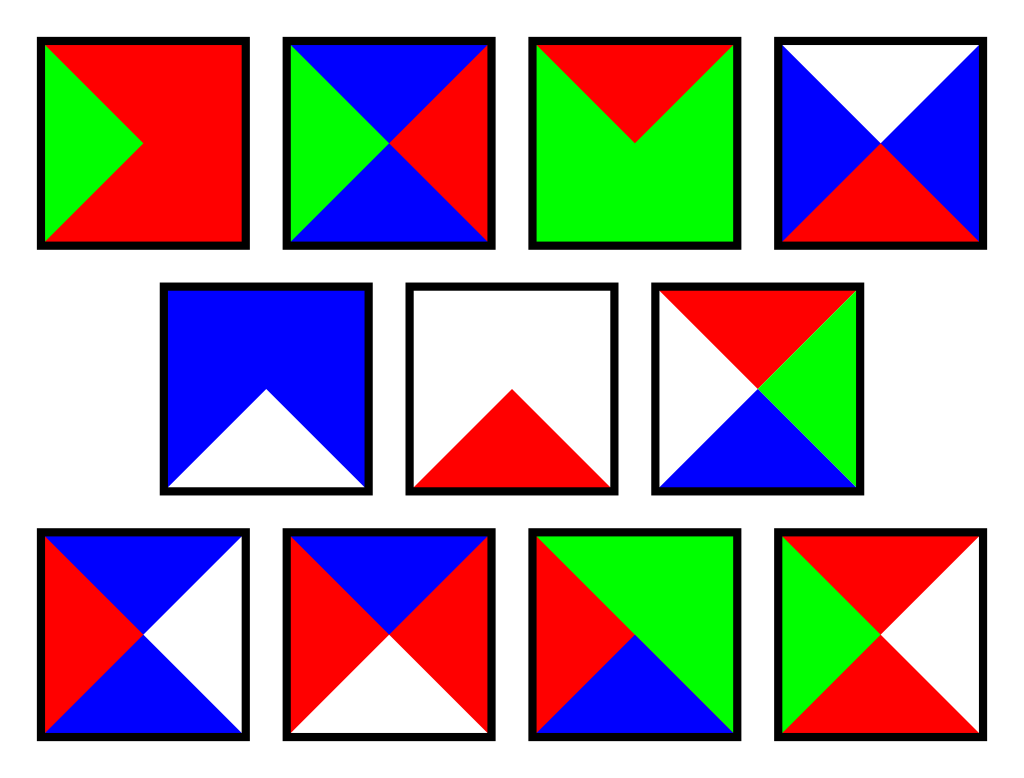
\includegraphics[scale=0.15]{img/Wang11.png}
				\caption{11 dominós}
				\label{fig: wang11}
			\end{figure}
			
		 \end{frame}
		 
		 \begin{frame}{ Dominó Wang}
			\justifying
			
			\begin{figure}[H]
				\centering
				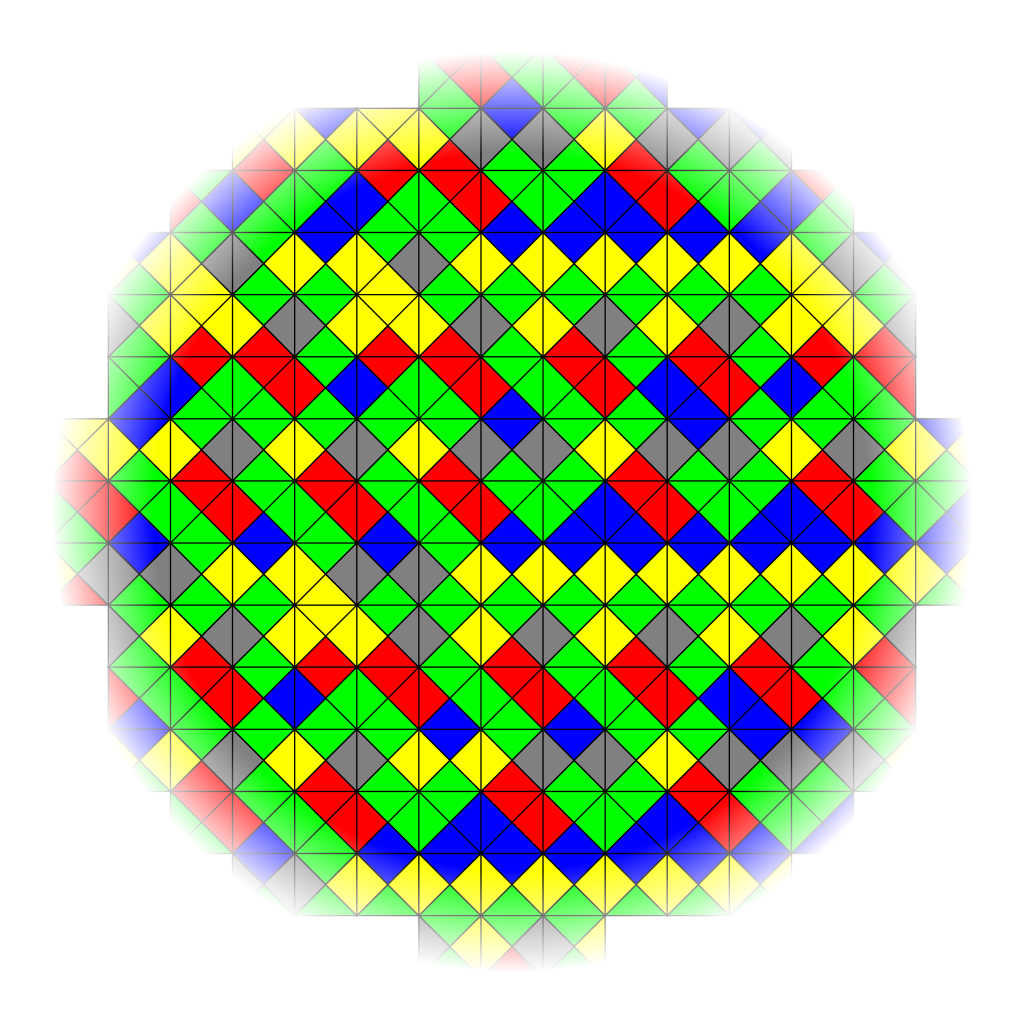
\includegraphics[scale=0.2]{img/Wangtess.png}
				\caption{13 dominós}
				\label{fig: wang13}
			\end{figure}
			
			
		 \end{frame}
		
		
		
	
	
	\section{Conclusiones}
		\begin{frame}{Conclusiones - Jerarquia de los lenguajes}
			\justifying
			\begin{figure}[H]
				\centering
				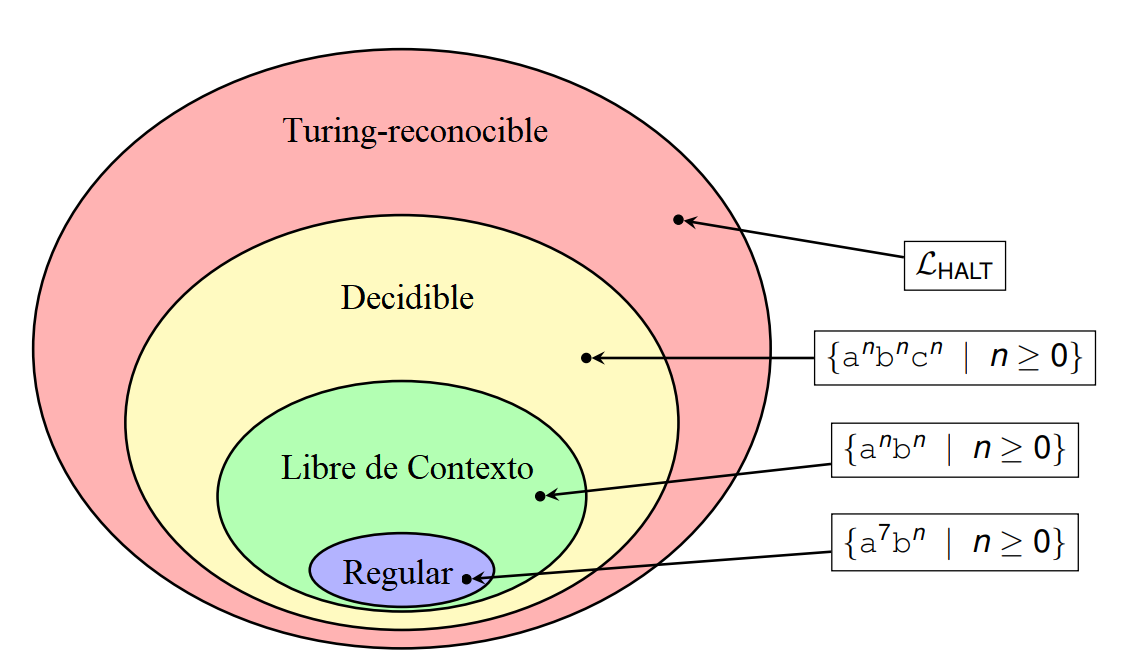
\includegraphics[scale=0.35]{img/jerarquiaLenguajes.PNG}
				\caption{L es una maquina de Turing-reconocible, ver que la jerarquía esta desde un lenguaje regular, lo que esta fuera es considerado un lenguaje indecidible}
				\label{fig: jeraquiaLenguajes}
			\end{figure}
		\end{frame}
		
		\begin{frame}{Conclusiones - Underfit es indecidible}
			\justifying
			
			\[ 
			    L_underfit = \{\langle A \rangle, d|A \in S, A \text{ underfits $d$ en todas la iteraciones}\} \text{es indecidible}
			\]
			
			\begin{figure}[H]
				\centering
				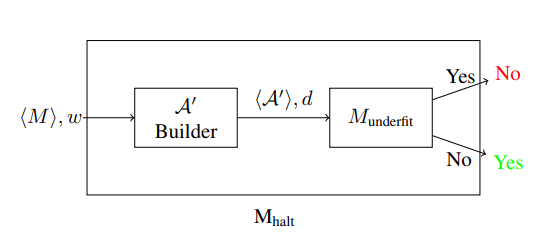
\includegraphics[scale=0.45]{img/underfit.PNG}
				\caption{
				Teorema que investigación que basado en el problema de Parada \cite{Sehra2021} define que un algoritmo de aprendizaje entraría en un estado underfit con ciertos dataset, pero esta investigación requiere ser reforzada con prueba de probabilidad para dar una validez}
				\label{fig: underfit}
			\end{figure}
			
			
			
		\end{frame}
		
		
	

	

%\appendix
\section{Referencias}
%\subsection<presentation>*{Referencias}

% All of the following is optional and typically not needed. 
%\appendix


\begin{frame}[t, allowframebreaks]
    \frametitle{References}
    \bibliographystyle{ieeetr}
    \bibliography{biblio}
\end{frame}
\end{document}